% #############################################################################    % This is the MAIN DOCUMENT of the IST-UL-Project-Report TEMPLATE. 
% !TEX root = ./main.tex
% #############################################################################
% The document is automatically set for english or portuguese by just selecting
% the MAIN LANGUAGE in file 'IST-UL-Project-Report-Preamble.tex' 
% #############################################################################
% Version 1.0, October 2018
% BY: Prof. Rui Santos Cruz, rui.s.cruz@tecnico.ulisboa.pt
% #############################################################################
%  Set the document class
% ----------------------------------------------------------------------
\documentclass[12pt,a4paper,oneside]{report}
% -----------------------------------------------------------------------------
% The Preamble document contains all the necessary Packages for typesetting
% Modify it to suit your needs
% -----------------------------------------------------------------------------
% #############################################################################
% Preamble for IST-UL-Project-Report in English or Portuguese
% Required Packages and commands
% --> Please Choose the MAIN LANGUAGE for the Thesis in package BABEL (below)
% !TEX root = ./main.tex
% #############################################################################
% Version 1.0, October 2018
% BY: Prof. Rui Santos Cruz, rui.s.cruz@tecnico.ulisboa.pt
% #############################################################################
% -----------------------------------------------------------------------------
% PACKAGE ucs:
% -----------------------------------------------------------------------------
% The 'ucs' package provides support for using UTF-8 in LaTeX documents. 
% However in most situations it is not required.
\usepackage{ucs}
% -----------------------------------------------------------------------------
% PACKAGE utf8x:
% -----------------------------------------------------------------------------
% The 'utf8x' package contains support for using UTF-8 as input encoding. 
\usepackage[utf8x]{inputenc}
% -----------------------------------------------------------------------------
% PACKAGE babel:
% -----------------------------------------------------------------------------
% The 'babel' package may correct some hyphenation issues of LaTeX. 
% Select your MAIN LANGUAGE for the Thesis with the 'main=' option.
% 
\usepackage[main=english,portuguese]{babel}
% -----------------------------------------------------------------------------
% PACKAGE iflang:
% -----------------------------------------------------------------------------
% The 'iflang' package is used to help determine the language being used. 
\usepackage{iflang}

% ----------------------------------------------------------------------
% Define default and cover page fonts.
% ----------------------------------------------------------------------
% Use Arial font as default
%
\renewcommand{\rmdefault}{phv}
\renewcommand{\sfdefault}{phv}
\def\FontLn{% 16 pt normal
  \usefont{T1}{phv}{m}{n}\fontsize{16pt}{16pt}\selectfont}
\def\FontLb{% 16 pt bold
  \usefont{T1}{phv}{b}{n}\fontsize{16pt}{16pt}\selectfont}
\def\FontMn{% 14 pt normal
  \usefont{T1}{phv}{m}{n}\fontsize{14pt}{14pt}\selectfont}
\def\FontMb{% 14 pt bold
  \usefont{T1}{phv}{b}{n}\fontsize{14pt}{14pt}\selectfont}
\def\FontSn{% 12 pt normal
  \usefont{T1}{phv}{m}{n}\fontsize{12pt}{12pt}\selectfont}
% ----------------------------------------------------------------------
% Define page margins and line spacing.
% ----------------------------------------------------------------------
% > set the page margins (2.5cm minimum in every side, as per IST rules)
%
\usepackage{geometry}	
\geometry{verbose,tmargin=2.5cm,bmargin=2.5cm,lmargin=2.5cm,rmargin=2.5cm}
%
% > allow setting line spacing (line spacing of 1.5, as per IST rules)
%
\usepackage{setspace}
\renewcommand{\baselinestretch}{1.5}
% ----------------------------------------------------------------------
% Include external packages.
\usepackage{graphicx}
\usepackage{amsmath}  % AMS mathematical facilities for LaTeX.
\usepackage{amsthm}   % Typesetting theorems (AMS style).
\usepackage{amsfonts} % 
\usepackage{subfigure}
\usepackage{subfigmat}
\usepackage{dcolumn}
\newcolumntype{d}{D{.}{.}{-1}} % column aligned by the point separator '.'
\newcolumntype{e}{D{E}{E}{-1}} % column aligned by the exponent 'E'
\usepackage[pdftex]{hyperref} % enhance documents that are to be
                              % output as HTML and PDF
\hypersetup{colorlinks,       % color text of links and anchors,
                              % eliminates borders around links
            linkcolor=blue,  % color for normal internal links
            anchorcolor=black,% color for anchor text
            citecolor=cyan,  % color for bibliographical citations
            filecolor=black,  % color for URLs which open local files
            menucolor=black,  % color for Acrobat menu items
            urlcolor=teal,   % color for linked URLs
	        bookmarksopen=true,    % don't expand bookmarks
	        bookmarksnumbered=true, % number bookmarks
            }
\usepackage[figure,table]{hypcap}
\usepackage[format=hang,labelfont=bf,font=small]{caption} 
\captionsetup[table]{skip=10pt}
\usepackage{cite}
\usepackage[printonlyused]{acronym}
\usepackage{lipsum}
\usepackage{tabularx}

% -----------------------------------------------------------------------------
% PACKAGE Cleveref:
% -----------------------------------------------------------------------------
% Clever Referencing of document parts
% Note: portuguese is supported through "brazilian" option
\usepackage[\IfLanguageName{english}{english}{brazilian}]{cleveref}
% -----------------------------------------------------------------------------
% PACKAGES xcolor, color
% -----------------------------------------------------------------------------
% These packages are required for list code snippets.
\usepackage{xcolor}
\usepackage{color}
% The following special color definitions are used in the IST Thesis
\definecolor{forestgreen}{RGB}{34,139,34}
\definecolor{orangered}{RGB}{239,134,64}
\definecolor{lightred}{rgb}{1,0.4,0.5}
\definecolor{orange}{rgb}{1,0.45,0.13}	
\definecolor{darkblue}{rgb}{0.0,0.0,0.6}
\definecolor{lightblue}{rgb}{0.1,0.57,0.7}
\definecolor{gray}{rgb}{0.4,0.4,0.4}
\definecolor{lightgray}{rgb}{0.95, 0.95, 0.95}
\definecolor{darkgray}{rgb}{0.4, 0.4, 0.4}
\definecolor{editorGray}{rgb}{0.95, 0.95, 0.95}
\definecolor{editorOcher}{rgb}{1, 0.5, 0} % #FF7F00 -> rgb(239, 169, 0)
\definecolor{chaptergrey}{rgb}{0.6,0.6,0.6}
\definecolor{editorGreen}{rgb}{0, 0.5, 0} % #007C00 -> rgb(0, 124, 0)
\definecolor{olive}{rgb}{0.17,0.59,0.20}
\definecolor{brown}{rgb}{0.69,0.31,0.31}
\definecolor{purple}{rgb}{0.38,0.18,0.81}




\usepackage{listings}
\lstset{escapeinside={<@}{@>}}
\usepackage{minted}

\lstdefinestyle{commandline} {%
language={[WinXP]command.com},
breaklines=true,
%aboveskip=\baselineskip,
belowskip=\baselineskip,
showstringspaces=false,
backgroundcolor=\color{black},
basicstyle=\small\color{white}\ttfamily
showstringspaces=false,
keywordstyle=\color{cyan}\bfseries,
stringstyle=\color{gray}\ttfamily,
commentstyle=\color{green}\itshape,
moredelim=[s][\color{yellow}\bfseries]{C:}{\>}
}

\lstdefinestyle{Bash} {%
language=bash,
breaklines=true,
belowskip=\baselineskip,
backgroundcolor=\color{lightgray},
showstringspaces=false,
keywordstyle=\color{black}\bfseries,
basicstyle=\small\color{black}\ttfamily,
stringstyle=\color{editorOcher}\ttfamily,
commentstyle=\color{brown}\itshape,
otherkeywords={xcode-select, mkdir,rm},
moredelim=[s][\color{darkblue}]{~$},
literate={~} {$\sim$}{1}
}

\lstdefinestyle{Rubytext} {%
language=Ruby,
breaklines=true,
belowskip=\baselineskip,
basicstyle=\small\ttfamily\color{black},
backgroundcolor=\color{lightgray},
showstringspaces=false,
commentstyle = \ttfamily\color{red},
keywordstyle=\ttfamily\color{blue},
stringstyle=\color{orange}
}
\lstset{escapeinside={<@}{@>}}

\lstdefinestyle{py} {%
	language=python,
	literate=%
	*{0}{{{\color{red}0}}}1
	{1}{{{\color{red}1}}}1
	{2}{{{\color{red}2}}}1
	{3}{{{\color{red}3}}}1
	{4}{{{\color{red}4}}}1
	{5}{{{\color{red}5}}}1
	{6}{{{\color{red}6}}}1
	{7}{{{\color{red}7}}}1
	{8}{{{\color{red}8}}}1
	{9}{{{\color{red}9}}}1,
	basicstyle=\small\ttfamily,
	numbers=left,
	% numberstyle=\tiny,
	% stepnumber=2,
	numbersep=5pt,
	tabsize=4,
	extendedchars=true,
	breaklines=true,
	keywordstyle=\color{blue}\bfseries,
	frame=b,
	commentstyle=\color{brown}\itshape,
	stringstyle=\color{editorOcher}\ttfamily,
	showspaces=false,
	showtabs=false,
	xleftmargin=17pt,
	framexleftmargin=17pt,
	framexrightmargin=5pt,
	framexbottommargin=4pt,
	backgroundcolor=\color{lightgray},
	showstringspaces=false,
}










% DEFINE COMMAND FOR: Acronyms listing Title depending on language
\newcommand{\tlangAcronyms}{\IfLanguageName{english}{Acronyms}{Acr\'onimos}}
% DEFINE COMMAND FOR: Degree Title depending on language
\newcommand{\tlangDegree}{\IfLanguageName{english}{Information Systems and Computer Engineering}{Engenharia Informática e de Computadores}}
% DEFINE COMMAND FOR: Course Title depending on language
\newcommand{\tlangCourse}{\IfLanguageName{english}{Management and Administration of IT Infrastrutures and Services}{Administração e Gestão de Infraestruturas e Serviços de IT}}
%%%%%%%%%%%%%%%%%%%%%%%%%%%%%%%%%%%%%%%%%%%%%%%%%%%%%%%%%%%%%%%%%%%%%%%%



% #############################################################################
\begin{document}
% Set plain page style (no headers, footer with centered page number)
\pagestyle{plain}
% Set roman numbering (i,ii,...) before the start of chapters
\pagenumbering{roman}
% ----------------------------------------------------------------------------
%  Cover page
% #############################################################################     % This is the FRONT COVER of the IST-UL-Project-Report TEMPLATE. 
% !TEX root = ./main.tex
% #############################################################################
% Version 1.0, October 2018
% BY: Prof. Rui Santos Cruz, rui.s.cruz@tecnico.ulisboa.pt
% #############################################################################
% #############################################################################
% DO NOT CHANGE THE FOLLOWING 4 LINES
\thispagestyle {empty}

\includegraphics[width=5cm]{./pictures/IST_A_RGB_POS.png}
\begin{center}
\vspace{5.0cm}
% #############################################################################
% #############################################################################
%
% INSERT THE TITLE OF THE PROJECT HERE
{\FontLb A Scalable Microservices-based Web Application in a
Public Cloud} \\
\vspace{0.2cm}
%
% INSERT THE SUBTITLE OF THE REPORT HERE
{\FontMn Capstone Project} \\
\vspace{1.0cm}
{\FontLn \tlangCourse} \\
\vspace*{1.0cm}
\begin{center}
\begin{tabular}{r@{~}l l}
    \multicolumn{3}{c}{\bfseries\textbf{ }} \\
    % INSERT YOUR TEAM NUMBER HERE
    & \textbf{Team nr.}: & 39 \\
    % INSERT IDs and NAMES of STUDENTS 
    & 87704: & Samuel Vicente \\
    & 86392: & Bruno Dias \\
    & 92510: & Lúcia Silva \\ % Comment if not necessary
\end{tabular}
\end{center}
\vspace*{2.0cm}
{\FontMb \tlangDegree} \\
{\FontMb IST-ALAMEDA} \\
\vspace{1.5cm}
{\FontMb 2021/2022} \\
\end{center}
\cleardoublepage
% ----------------------------------------------------------------------------
%  Table of contents, list of tables, list of figures and nomenclature
% ----------------------------------------------------------------------------
\tableofcontents
\clearpage 
\begingroup 
    \let\clearpage\relax
    \let\cleardoublepage\relax
    \let\cleardoublepage\relax
% List of tables
\listoftables
% Add entry in the table of contents as section
\addcontentsline{toc}{section}{\listtablename}
% List of figures
\listoffigures
% Add entry in the table of contents as section
\addcontentsline{toc}{section}{\listfigurename}
\endgroup
\chapter*{\tlangAcronyms}
\begin{acronym}[NGOSS]
	\acro{GCP}{Google Cloud Platform}
	\acro{GKE}{Google Kubernetes Engine}
	\acro{GCE}{Google Compute Engine}
	\acro{K8S}{Kubernetes}
	\acro{IaC}{Infrastructure as Code}
	\acro{GAR}{Google Artifact Registry}
	\acro{MS}{Micro Services}
	\acro{IP}{Internet Protocol}
	\acro{VPC}{Virtual Private Cloud}
	\acro{CI}{Continuous Integration}
	\acro{CD}{Continuous Deployment}
	\acro{JSON}{JavaScript Object Notation}
	\acro{URL}{Uniform Resource Locator}
	\acro{API}{Application Programming Interface}
\end{acronym}
% Set arabic numbering (1,2,...) after preface
\setcounter{page}{1}
\pagenumbering{arabic}
% #############################################################################
%
%                           BEGIN MAIN DOCUMENT BODY
%
% #############################################################################
\chapter{Introduction}
\label{chapter:introduction}
This project describes the process of deploying and provisioning a micro services based containerized web application in a public cloud provider, in our case, \ac{GCP}, using \ac{IaC} tool \href{https://www.terraform.io/}{Terraform}.

The application to be deployed, \href{https://github.com/khandelwal-arpit/kubernetes-starterkit}{Kubernetes Starterkit}, is a simple browser-based calculator, using multiple distinct technologies, with a simple frontend and 
three backend services that provide the calculator operations (addition, multiplication, etc) and the executed operations history:

\begin{itemize}
  \item Vuecalc service (Vue.js);
  \item Expressed service (Express.js);
  \item Happy service (Hapi.js);
  \item Bootstorage service (Java Spring Boot);
\end{itemize}

Vuecalc is a simple calculator UI frontend application that uses the endpoints exposed by the Expressed, Happy and Bootstorage backend applications. Happy provides multiplication and division capabilities while Expressed provides addition and subtraction, both these services send the operations they execute to the bootstorage service in order to save the history of operations, this history can then be observed in the Vuecalc application.
Bootstorage is a simple service whose sole purpose is to store and return the operations executed in a \href{https://redis.io/}{Redis Data Store}.

Since the application was containerized, it made sense to use \ac{K8S} for automatic deployment and management of the application containers. \ac{GKE} was used to create the cluster and \ac{GAR} to manage and store container images.

A video over viewing the contents of this report is available \href{https://youtu.be/PeXhR1QCIVk}{here}.
\cleardoublepage

\cleardoublepage
\chapter{Methodology}
This chapter describes the architecture of the implementation as well as each of its components.
\section{Architecture}

\begin{figure}[htb]
\centering
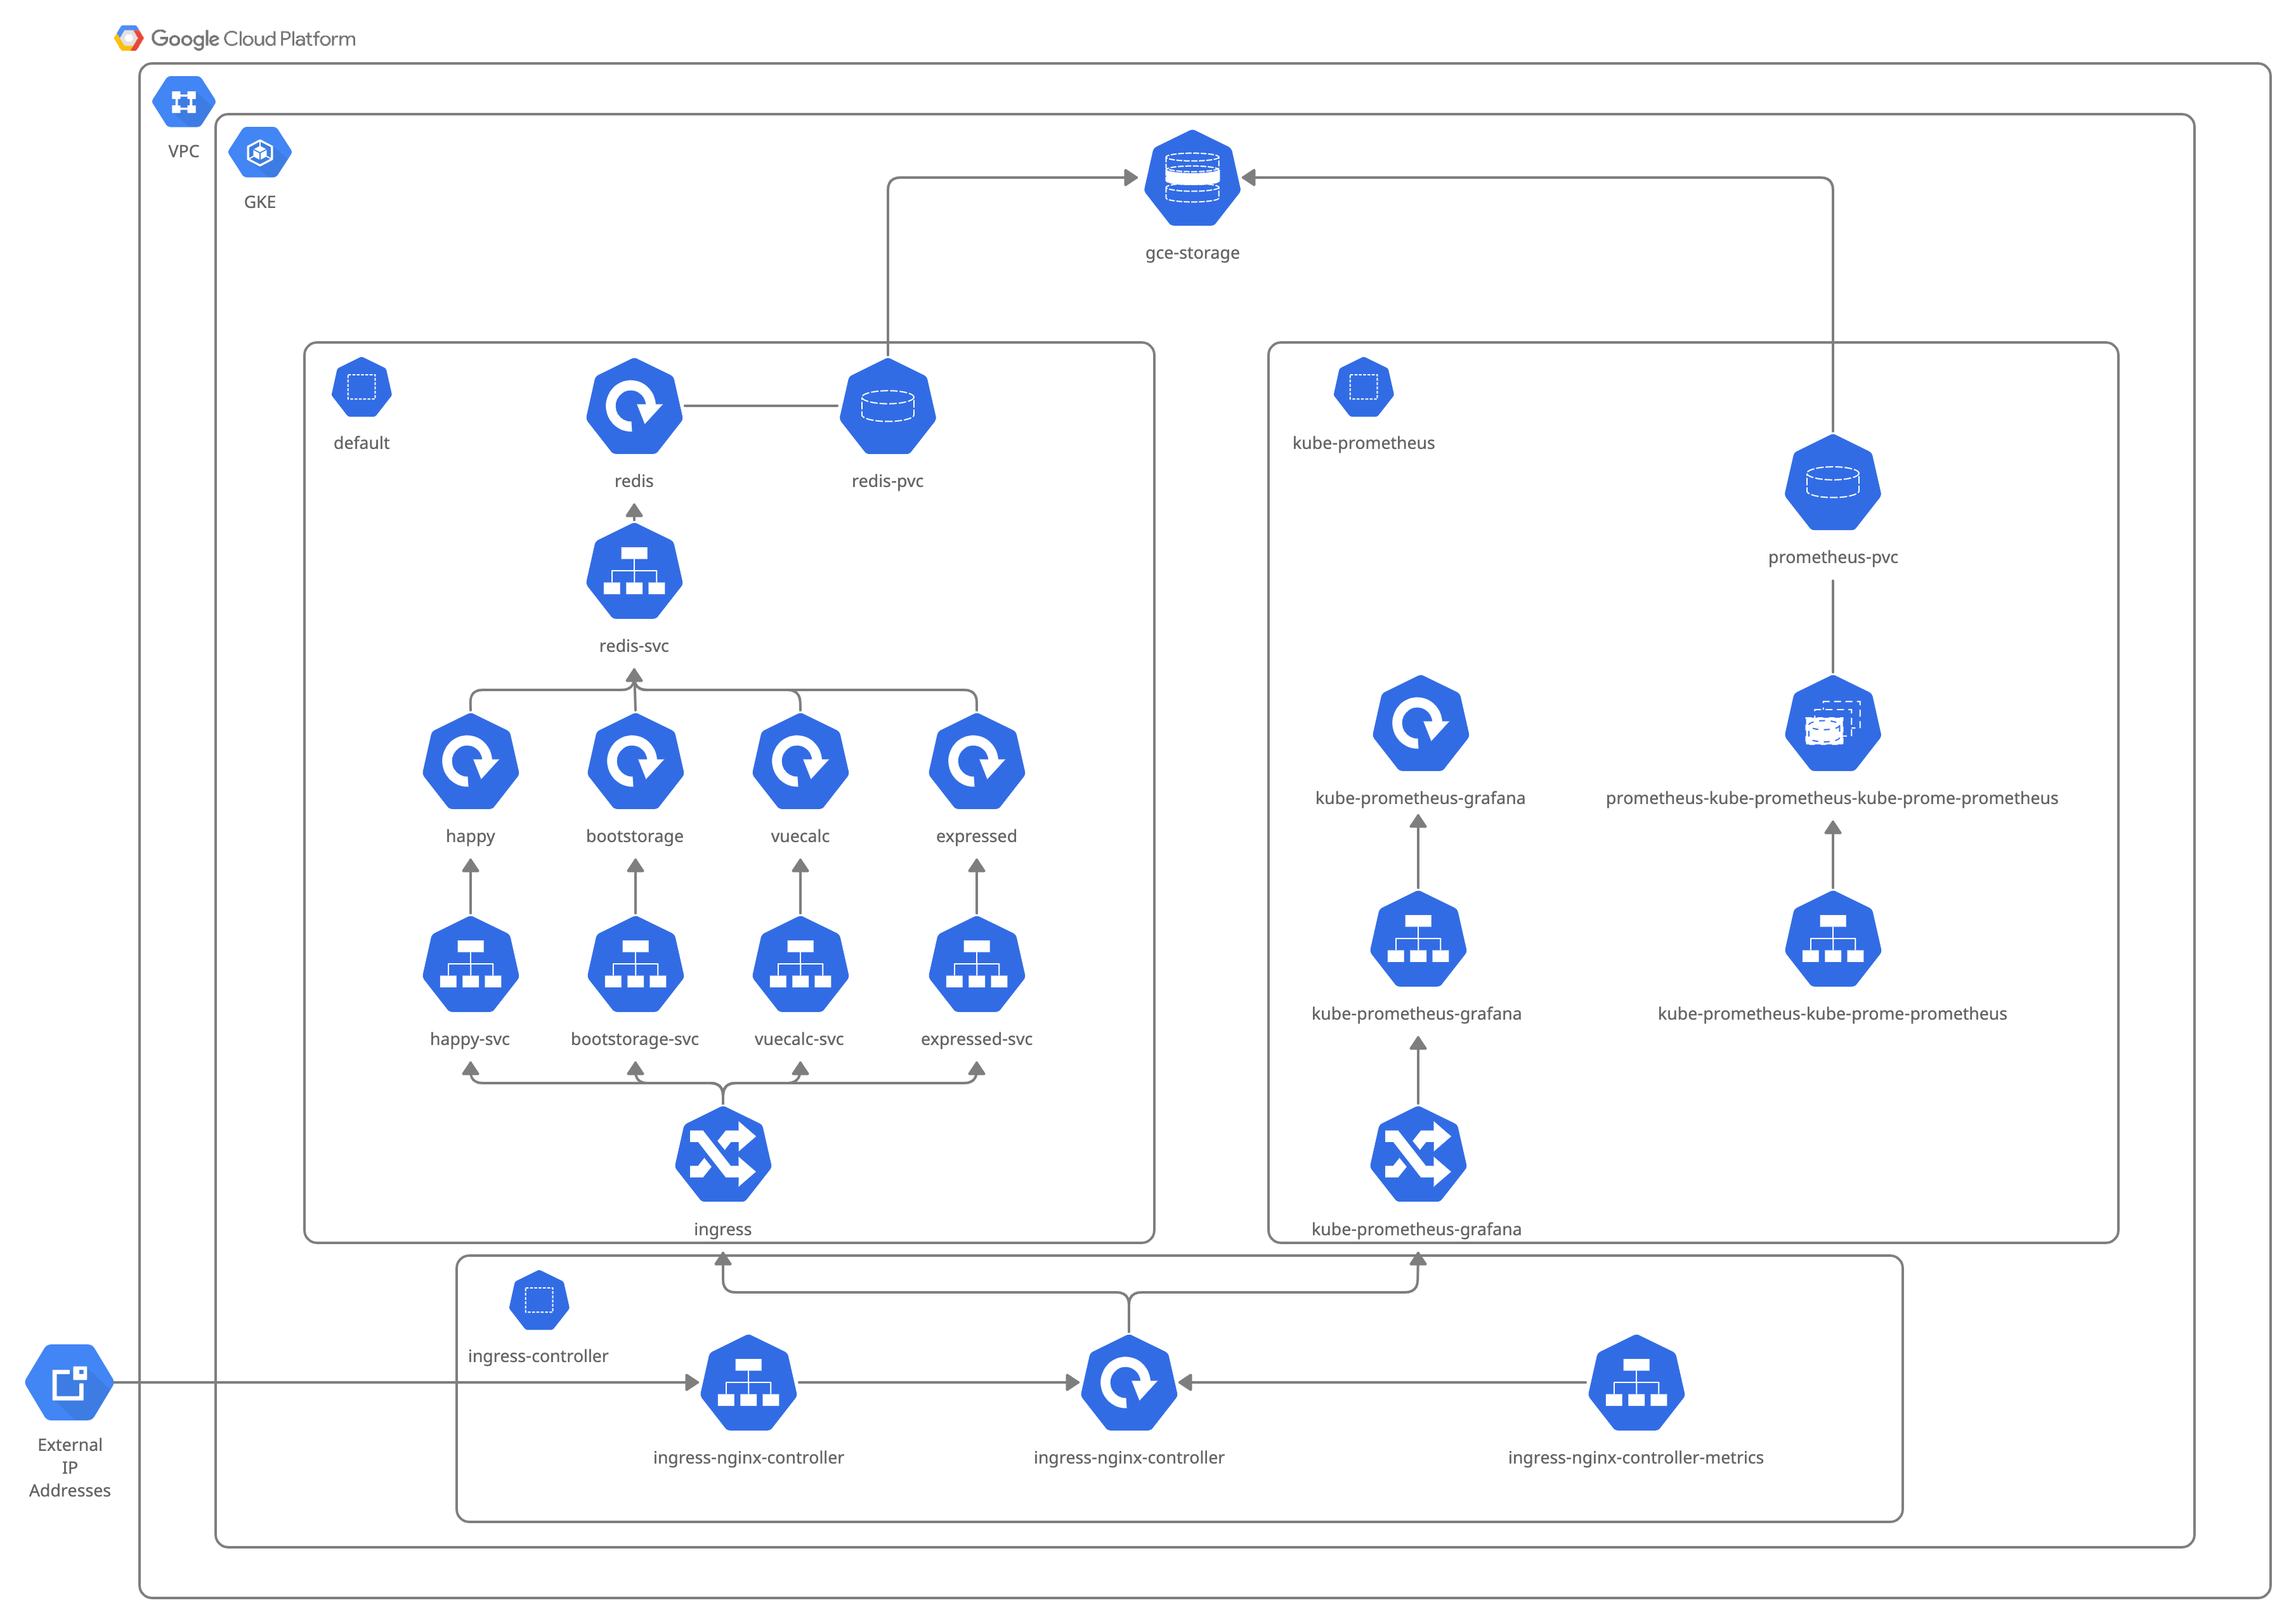
\includegraphics[width=1.0\textwidth]{./pictures/arch.png}
\caption{Solution architecture}
\label{fig:network}
\end{figure}

We chose to build our cluster using \ac{GKE}, this greatly simplifies the creation of the cluster. We deployed the cluster inside a \ac{VPC}.

We then defined a StorageClass to use with the applications that need persistent storage, in our case, Redis and Prometheus.

All our services are cluster internal, meaning they do not have external \ac{IP} addresses, this is by choice as we deemed better to use a reverse proxy to forward the requests from outside to inside the cluster. To accomplish this task we used the \href{https://kubernetes.github.io/ingress-nginx/}{NGINX Ingress Controller}. This serves as both the \ac{API} gateway and reverse proxy. We defined two ingresses, one for each namespace that needed it, the default namespace and the kube-prometheus namespace.
All the services inside the default namespace apart from the redis-svc are mapped to an \ac{API} path in ingress.
In the kube-prometheus namespace only the Grafana service is mapped to an \ac{API} path in ingress .

This diagram is a simplification of the actual component graph of our cluster, the kube-prometheus namespace, since it was deployed using a helm chart, deploys a lot of services and other components not pictured here.

\section{Components} 

In this subsection we describe the main parts of the solution such as the \ac{K8S} cluster itself, the alternative tool to dockerhub and all the deployments and services used, as well as the monitoring tools.

\subsection{K8S Cluster}
\ac{K8S} is an open-source container-orchestration system that automates the deployment, scaling, and administration of computer applications. 

\subsection{Artifact Registry}
Similarly to Docker Hub, \ac{GAR} allows the creation of a repository to manage and store docker images that can be deployed into the \ac{K8S} cluster. When planning the overall solution it made sense for the docker images to share the same project as the infrastructure, so that it has direct access and in future works a pipeline to automate the process including the build and containerization of the images could be implemented using tools provided by google such as Google Cloud Build, easing and automating the all process, providing a tool that allows \ac{CI} and \ac{CD} of the application, possibly the infrastructure itself.


\subsection{Application Deployments and Services}

Our application is composed by a set of deployments. 

A deployment is used to tell \ac{K8S} how to create or modify instances of the pods that hold a containerized application.

A pod is a group of one or more containers, that share storage/network resources, and a specification on how to run them.

A service is a logical abstraction for a deployed group of pods in a cluster. Since pods are ephemeral, a service enables a group of pods, that provide the same functionality, to be assigned a name and unique IP address. This way, since pods and its \ac{IP} are not permanent, the service serves as the abstraction of the group that is referenced by the service name, so that each time that a pod is replaced, it is still correctly referenced.

\par
The services used for the correct functioning of the application are those listed below:
\begin{itemize}
    \item \textbf{Vuecalc}:Allows interaction with the calculator functionalities.
    \item \textbf{Expressed}:Performs addition and subtraction operations.
    \item \textbf{Happy}:Performs division and multiplication operations.
    \item \textbf{Bootstorage}:Retrieves the data and operations performed upon the calculator.
    \item \textbf{Redis}:Serves as the data storage for the bootstorage service.
\end{itemize}



\subsection{Ingress}

The ingress is the entity responsible for managing the access to the cluster from the outside, exposing a single \ac{IP} for accessing the application services. Ingress has the ability to forward IP packets, from the client requests to the services requested. The following table specifies the routing for our cluster ingress:

\begin{table}[h]
\centering
  \caption{Routing Rules}
    \label{tab:Ingress}
\begin{tabularx}{0.8\textwidth} 
    { 
  | >{\raggedright\arraybackslash}X 
  | >{\centering\arraybackslash}X 
  | >{\raggedleft\arraybackslash}X | }

\hline
 Path & Service Name & Service Port\\
 \hline
 /   & Vuecalc    & 2000  \\
 \hline
 /api/express   & Expressed  & 3000  \\
 \hline
 /api/happy     & Happy  & 4000           \\
 \hline
 /api/bootstorage   & Bootstorage & 5000        \\
 \hline
  /grafana  & Grafana & 80        \\
 \hline
\end{tabularx}
\end{table}



\subsection{Monitoring}

For the purpose of monitoring the cluster, \href{https://github.com/prometheus-operator/kube-prometheus}{kube-prometheus} was used, this is a collection of Grafana dashboards and Prometheus rules combined with documentation and script, in order to provide easy to operate end-to-end \ac{K8S} cluster monitoring with Prometheus using the Prometheus Operator.

The Prometheus Operator includes a Custom Resource Definition that allows the definition of the ServiceMonitor, used to define in which applications, by specifying \ac{K8S} labels to each of the services, metrics shall be retrieved from within Kubernetes. The controller builds the required prometheus configurations.
Applications and services expose a HTTP endpoint that contains Prometheus formatted metrics, which Prometheus will retrieve.

With this, real-time metrics can be stored by Prometheus and afterwards visualized using Grafana in charts.



\cleardoublepage
\chapter{Implementation}
This chapter describes the project files, pre-requisites for deployment and the deployment procedure itself.
\section{Project Files}
\begin{lstlisting} [style=bash,caption={Structure of the team-39A/labs/project directory}]
team-39A/labs/project
		|-- README.md
		|-- build_push.sh
		|-- gcp
		|   |-- ...
		|-- microservices
		|   |-- ...
		|-- report
		|   |-- ...
		|-- demo
		|   |-- ...
\end{lstlisting}

This is the root folder of the project, here we find:
\begin{itemize}
    \item The build\_push.sh script: this script encompasses the setup of the \ac{GAR} repository and the building and pushing of the \ac{MS} images to said repository. This is only a convenience, in a real life scenario, this would not be acceptable and more appropriate tools like \href{https://www.jenkins.io/}{Jenkins} or \href{https://cloud.google.com/build}{Google Cloud Build} would be advised;
    \item gcp directory: Here is where all the Terraform files reside;
    \item microservices directory: Here is where all the code and Dockerfiles for the \ac{MS} reside; 
    \item report directory: Here is where the checkpoints and final reports are;
    \item demo directory: Here is where the demo guide is;
\end{itemize}

The main focus of this project was the /gcp directory and so, we will focus on that.

\begin{lstlisting} [style=bash,caption={Structure of the /gcp directory}]
gcp
    |-- gke
    |   |-- ...
    |-- k8s
    |   |-- ...
    |-- registry
    |   |-- ...
    |-- main.tf
    |-- terraform.tfvars
    |-- variables.tf*-
\end{lstlisting}

On this folder we have three modules, one for each step of the infrastructure deployment.
First the \ac{GAR} repository must be created in order to store the container images that we will use in the Kubernetes deployments. This is the purpose of the registry module, that resides in the registry directory. 

After that is created and the images are in there we can proceed to the creation of the \ac{K8S} cluster itself. This is the responsibility of the gke module, defined in the gke directory.

As soon as the cluster finishes creation we can start deploying in it. The k8s module, defined in the k8s directory, defines all the things to be deployed inside the cluster (services, deployments, secrets, etc).

As was previously stated the registry module is used by the build\_push.sh script and so was not included in the main.tf file.

The main.tf file is where the gke and k8s modules are configured and executed. 

\subsection{Registry module}
\subsubsection{Overview}
\begin{lstlisting} [style=bash,caption={Structure of the registry module}]
registry
    |-- provider.tf
    |-- registry.tf
    |-- variables.tf
\end{lstlisting}

In this module we define the \ac{GAR} repository, for Docker images.
In order to do this we must use the \href{https://registry.terraform.io/providers/hashicorp/google-beta/latest}{Terraform google-beta provider} as this feature is not available in the non beta provider. 

\subsubsection{Inputs}
This module needs the following information in order to execute:
\begin{itemize}
    \item The region where the cluster will be deployed;
    \item The project id where the repository will be deployed;
    \item Json key file for accessing \ac{GCP};
    \item The repository name/id;
\end{itemize}

\subsection{Gke module}
\subsubsection{Overview}
\begin{lstlisting} [style=bash,caption={Structure of the gke module}]
gke
    |-- cluster.tf
    |-- outputs.tf
    |-- provider.tf
    |-- templates
    |   |-- kubectl.tmpl
    |-- variables.tf
    |-- vpc.tf
\end{lstlisting}

In this module we define the \ac{K8S} cluster.
To do this we used \href{https://registry.terraform.io/providers/hashicorp/google/latest}{Terraform google provider}.

We first created a \ac{VPC} network, by default \ac{GCP} blocks all access from outside this network, effectively separating our cluster from the internet, when we add resources to this network, for instance, the cluster, \ac{GKE} creates the necessary firewall rules in order to allow communication with the kube-apiserver, or ingress endpoint. We then define a subnetwork of this network with two \ac{IP} ranges, one for the pods and another for the services.

Now that we have the \ac{VPC} network we can define the cluster itself.

This cluster will be deployed in the network created and the subnetwork's \ac{IP} ranges allocated to the services and pods. Unlike in the labs, we opted to create a separate node pool, this enables us to add or remove nodes without having to redeploy the entire cluster.

\subsubsection{Inputs}
This module needs the following information in order to execute:
\begin{itemize}
    \item The region where the cluster will be deployed;
    \item The zone where the cluster will be deployed;
    \item Json key file for accessing the google cloud;
    \item The project id where the cluster will be deployed;
    \item Number of worker nodes for the cluster;
    \item Type of machine to use for the kubernetes nodes;
    \item A map of ip ranges for the pods and services;
\end{itemize}

\subsubsection{Outputs}
We output the following values out of the module:
\begin{itemize}
    \item The IP address of the cluster's Kubernetes master;
    \item The private key used by clients to authenticate to the cluster endpoint;
    \item The public certificate used by clients to authenticate to the cluster endpoint;
    \item The public certificate that is the root of trust for the cluster;
\end{itemize}

This module creates a shell script with the necessary gcloud command to configure kubectl for the local machine. This is for convenience.

\subsection{K8S module}
\subsubsection{Overview}
\begin{lstlisting} [style=bash,caption={Structure of the k8s module}]
k8s
    |-- bootstorage.tf
    |-- expressed.tf
    |-- happy.tf
    |-- ingress.tf
    |-- monitoring.tf
    |-- output.tf
    |-- provider.tf
    |-- pv.tf
    |-- redis.tf
    |-- resources
    |   |-- nginxdash.json
    |-- templates
    |   |-- ingress-nginx.tmpl
    |   |-- ingressIP.tmpl
    |   |-- kube-prometheus-stack.tmpl
    |-- variables.tf
    |-- vuecalc.tf
\end{lstlisting}

In this module we define the things that will get deployed in the cluster.
To do this we used \href{https://registry.terraform.io/providers/hashicorp/kubernetes/latest}{Terraform google provider} and \href{https://registry.terraform.io/providers/hashicorp/helm/latest}{Terraform helm provider}.

We can divide these files into 4 categories:
\begin{itemize}
	\item Monitoring:
		\begin{itemize}
			\item monitoring.tf;
			
        		The monitoring stack used was the \href{https://github.com/prometheus-community/helm-charts/tree/main/charts/kube-prometheus-stack}{kube-prometheus-stack helm chart} that provides us with a simple way of deploying and configuring the monitoring stack. 
			
        		This chart was deployed in the kube-prometheus namespace. 
        		
        		By default this chart does not configure the monitoring for the ingress-nginx controller, so we had to add this capability. To do so we had to set a value so that Prometheus goes looking for serviceMonitors outside the helm specified namespace. We also added a persistent volume to Prometheus.
        		
        		Since ingress-nginx is not supported by default we also had to add an additional grafana dashboard to view the data gathered by Prometheus. We did this by defining a configMap  with the \ac{JSON} definition of the dashboard. Grafana is configured to used configMaps that have a specified labels in their metadata. 
        		
        		We also configure Grafana to enable Ingress on the /grafana path and to use the nginx controller.

		\end{itemize}
		
	\item Micro Services:
	
	    These files define the deployments and services of our application.
	    
	    All the services are of type ClusterIP as we do not want to expose them directly to outside the cluster.
	    
	    All the deployments have startup, readiness and liveness probes and one replica.
	    
	    All the components of this category are defined inside the default namespace.
	    
	
		\begin{itemize}
			\item bootstorage.tf;
			
			Here we define the bootstorage service and deployment. We also define a secret for bootstorage to use when connecting with the Redis service. 
			
			\item vuecalc.tf;
			
			Here we define the vuecalc service and deployment.
		    For this deployment the application requires us to define the base \ac{URL} for the multiple \ac{API} we offer. To do this we needed to set multiple environment variables.
			
			\item happy.tf;
			
			Here we define the happy service and deployment.
			
			\item expressed.tf;
			
			Here we define the bootstorage service and deployment.
		\end{itemize}
	\item Storage: 
		\begin{itemize}
			\item pv.tf;
			
			    Here we define the storageClass and the persistentVolumeClaim for the redis deployment.
			    The storageClass is provisioned by \ac{GCE} and is of type pd-ssd. The reclaim policy is retain so that the storage does not get deleted when it is released.
			    
			\item redis.tf;
			
			    In this file we define the redis deployment of one replica. 
			    
			    We specify the startup args so that redis will periodically dump to disk its internal state.
			    We give it the volume claimed to mount on the /data directory.
			    
			    We also define a headless service, a service with no clusterIP that instead will return the ip of the pod running the application, in this case, Redis. 
		\end{itemize}
	\item Ingress:
		\begin{itemize}
			\item ingress.tf;
			
			In order to access our services, which only have an internal clusterIP we must expose them through Ingress. We could do this only using it as an \ac{API} gateway with the cloud provider controller doing the work, meaning that we would have to expose the services to outside the cluster, or we could define the controller ourselves inside the cluster meaning that along with the \ac{API} gateway functionality we could also use it as a reverse proxy. We chose the latter. 
			
			Our ingress controller of choice was the nginx-ingress-controller. We deployed it making use of the \href{https://artifacthub.io/packages/helm/ingress-nginx/ingress-nginx}{ingress-nginx helm chart}.
			
			The controller was deployed inside its own namespace ingress-controller.
			
			Since we wanted to gather metrics about the controller we had to enable that functionality.
			
			In this file we also define the Ingress for the services the application offers, this Ingress is defined in the default namespace, where the services are defined. We must state in the Ingress metadata for it to use the nginx controller.
			
			
		\end{itemize}
\end{itemize}

\subsubsection{Inputs}
This module needs the following information in order to execute:
\begin{itemize}
    \item The IP address of the cluster's Kubernetes master;
    \item The private key used by clients to authenticate to the cluster endpoint;
    \item The public certificate used by clients to authenticate to the cluster endpoint;
    \item The public certificate that is the root of trust for the cluster;
    \item The region where the image repository is deployed;
    \item The project id where image repository is deployed;
    \item The Grafana access password for the admin user;
\end{itemize}

\subsubsection{Outputs}
This module creates a markdown file with the \ac{IP} address of the ingress created.
\clearpage
\section{Deployment}

The next subsections describe the steps needed to correctly deploy and configure the \ac{MS} application into the \ac{K8S} cluster. 

First we will go through all the necessary pre-requisites, followed by the creation of a repository to store the docker images, and lastly the infrastructure provisioning and deployment.



\subsection{Pre-requisites}
In order to deploy our project there is a set of requirements that must be met.

First, lets overview what software needs to be installed in the machine that will preform the deployment. All software used was on the latest version as of November 2021;
\begin{itemize}
\item Terraform;
\item Docker Engine;
\item npm;
\item JDK8;
\item maven;
\item gcloud;
\item awk;
\item bash;
\end{itemize}

Now that the required software is installed we can move on to setting up the \ac{GCP} environment:
\begin{enumerate}
\item Create a new project;
\item Enable \ac{GKE} API;
\item Enable \ac{GAR} API;
\item Add Kubernetes Engine Service Agent Role to the Compute Engine default service account;
\item Create new key for the Compute Engine default service account, in the JSON format;
\item Save this key in the /project/gcp directory;
\end{enumerate}

We can now set up the /project/gcp/terraform.tfvars file with the missing values, or change the already present ones.
\begin{lstlisting} [style=bash,caption={terraform.tfvars}]
region       = "europe-west1"
zone         = "b"
project      = "<PROJECT_ID>"
credentials  = "<JSON_KEY_PATH>"
node_count   = 3
machine_type = "n1-standard-2"
secondary_ip_ranges = {
"pod_ip_range"      = "10.0.0.0/14"
"services_ip_range" = "10.4.0.0/19"
}
registry = "myrepo" # GAR repository ID to be created
grafana_password = "grafanamonitoring"
\end{lstlisting}

For a more detailed step-by-step please refer to the \href{https://youtu.be/PeXhR1QCIVk?t=267}{video} that accompanies this report.

\subsection{Artifact Registry Repository Creation}

In order to proceed to the repository creation using \ac{GAR}, a script located in the root of the project called \texttt{build\char`_push.sh} was created, responsible for:

\begin{itemize}
\item Authenticating with gcloud;
\item Setting the project in gcloud;
\item Create the \ac{GAR} repository in the \ac{GCP} project;
\item Configure Docker to use this repository;
\item Build the \ac{MS} images and push them to this repository;
\end{itemize}

\begin{lstlisting} [style=bash]
$ ./build_push.sh
\end{lstlisting}

\begin{figure}[htb]
\centering
  \centering
  {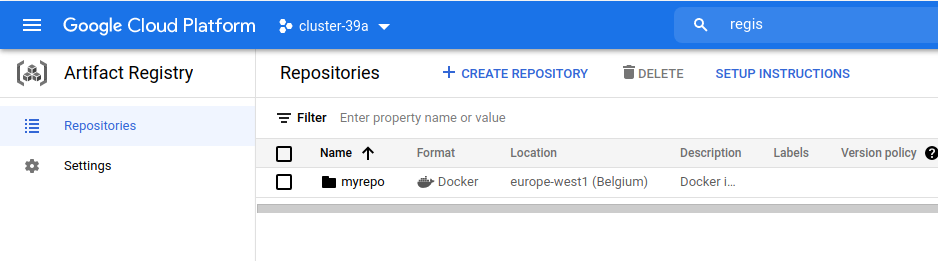
\includegraphics[width=0.4\textwidth]{./pictures/repo.png}}
  \hfill
  {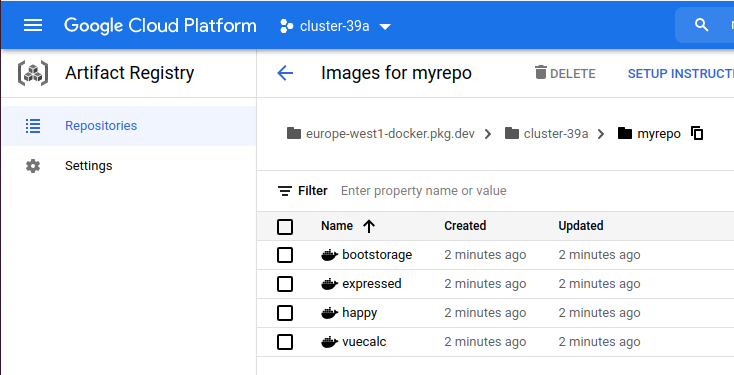
\includegraphics[width=0.4\textwidth]{./pictures/repofiles.png}}
\caption{Google Artifact Registry}
\label{fig:Artifact Registry}
\end{figure}


\subsection{K8S cluster Provisioning and Deployment}

Go to the /project/gcp directory of the project and follow the following steps:

The following commands create and provision the infrastructure. The outputs obtained should be similar to the ones presented.

\begin{lstlisting} [style=bash]
$ terraform init
\end{lstlisting}

\begin{figure}[H]
\centering
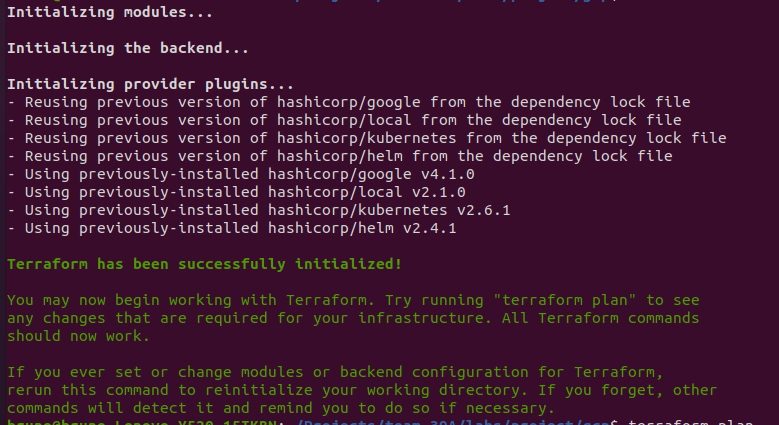
\includegraphics[width=1\textwidth]{./pictures/init.png}
\caption{Terraform Init}
\label{fig:Terraform Init}
\end{figure}

\begin{lstlisting} [style=bash]
$ terraform plan
\end{lstlisting}

\begin{figure}[H]
\centering
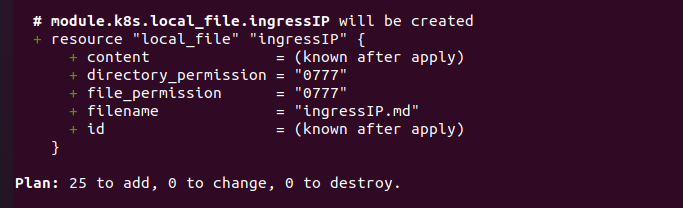
\includegraphics[width=1.0\textwidth]{./pictures/plan.png}
\caption{Terraform Plan}
\label{fig:Terraform Plan}
\end{figure}


\begin{lstlisting} [style=bash]
$ terraform apply auto-approve
\end{lstlisting}

\begin{figure}[H]
\centering
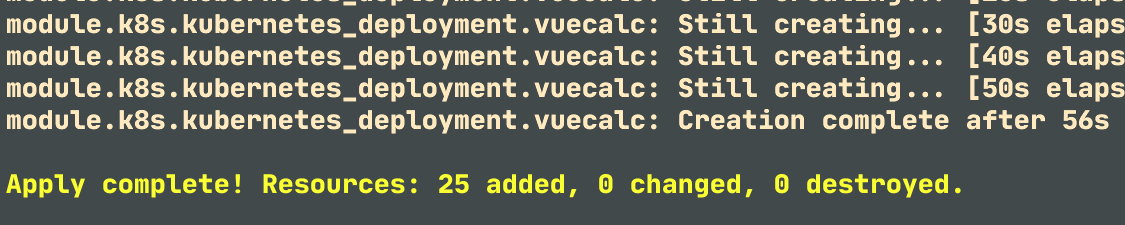
\includegraphics[width=1.0\textwidth]{./pictures/apply.png}
\caption{Terraform Apply}
\label{fig:Terraform Apply}
\end{figure}


\begin{itemize}
    \item Now, in order to access the cluster and run commands, kubectl is used, and can be configured with the following command. Zone and ProjectID correspond to your project's specifications.
    
    Alternatively we can run the kubectl.sh file in the /gcp directory that already has these values set. 
    
\end{itemize}
\begin{lstlisting} [style=bash]
$ gcloud container clusters get-credentials vpc-native-cluster --zone <Zone> --project <ProjectId>
\end{lstlisting}

\begin{lstlisting} [style=bash]
$ ./kubectl.sh
Fetching cluster endpoint and auth data.
kubeconfig entry generated for vpc-native-cluster.
\end{lstlisting}

\begin{itemize}
    \item Using kubectl, the namespaces can be retrieved.
\end{itemize}

\begin{lstlisting} [style=bash]
$ kubectl get namespaces
\end{lstlisting}

\begin{figure}[H]
\centering
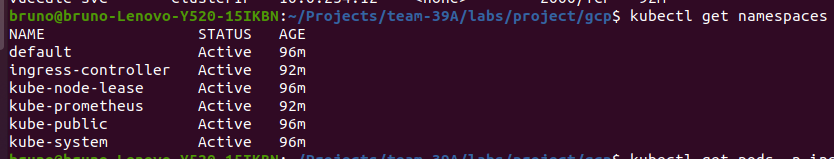
\includegraphics[width=1.0\textwidth]{./pictures/namespaces.png}
\caption{Cluster namespaces}
\label{fig:Cluster namespaces}
\end{figure}


\begin{itemize}
    \item Check default namespace, namespace in which our microservices app is located, with which it is displayed all the components, particularly the pods and services referring to it.
    
    As we can see in figure \ref{fig:Application  namespace}, none of the components is exposed to the internet.
\end{itemize}
\begin{lstlisting} [style=bash]
$ kubectl get all -n default
\end{lstlisting}

\begin{figure}[H]
\centering
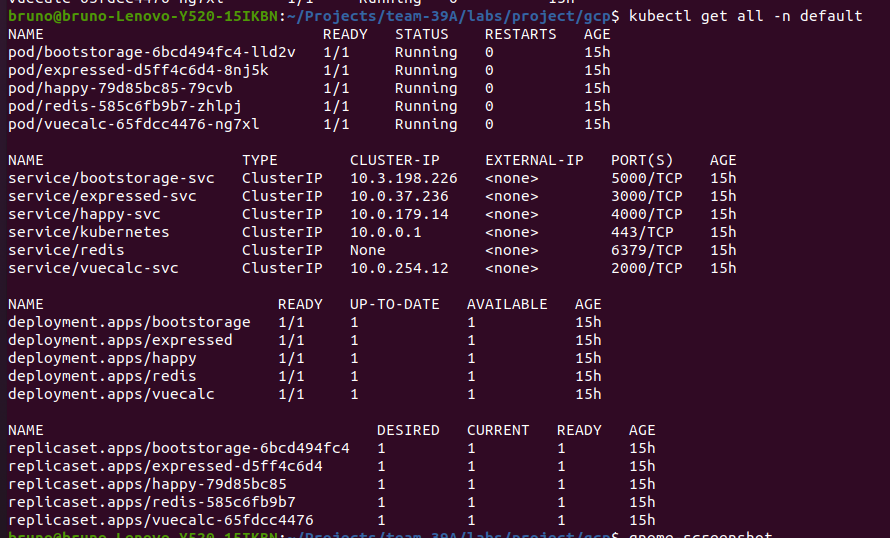
\includegraphics[width=1.0\textwidth]{./pictures/deafult.png}
\caption{Application namespace}
\label{fig:Application  namespace}
\end{figure}
\begin{itemize}
    \item In order to access the application, we need to retrieve the \ac{IP} exposed by the Ingress and we can get it by looking at the correspondent namespace. In the services, the nginx-controller exposes an \ac{IP}. 
    
    Alternatively we can cat the ingressIP.md file in the /gcp directory that already has external \ac{IP} of the Ingress endpoint. 
\end{itemize}
\begin{lstlisting} [style=bash]
$ kubectl get all -n ingress-controller
\end{lstlisting}

\begin{lstlisting} [style=bash]
$ cat ingressIP.md
# Ingress IP address:
34.79.197.230
\end{lstlisting}

\begin{figure}[H]
\centering
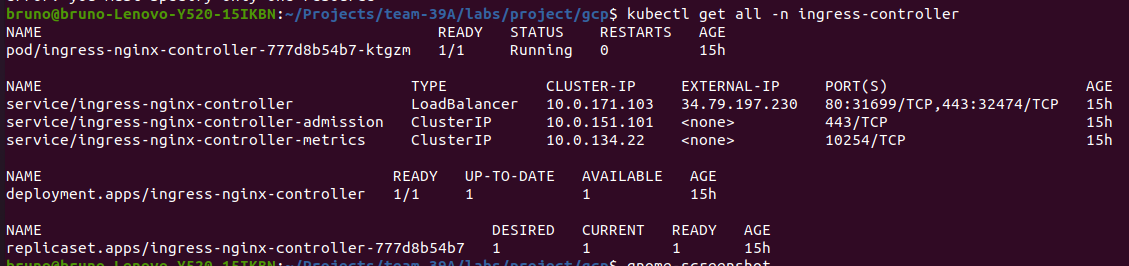
\includegraphics[width=1.0\textwidth]{./pictures/ingrrr.png}
\caption{Ingress}
\label{fig:Ingress}
\end{figure}

\begin{itemize}
    \item We then copy the correspondent \ac{IP} to a browser and we can access the application UI.
\end{itemize}

\begin{figure}[H]
\centering
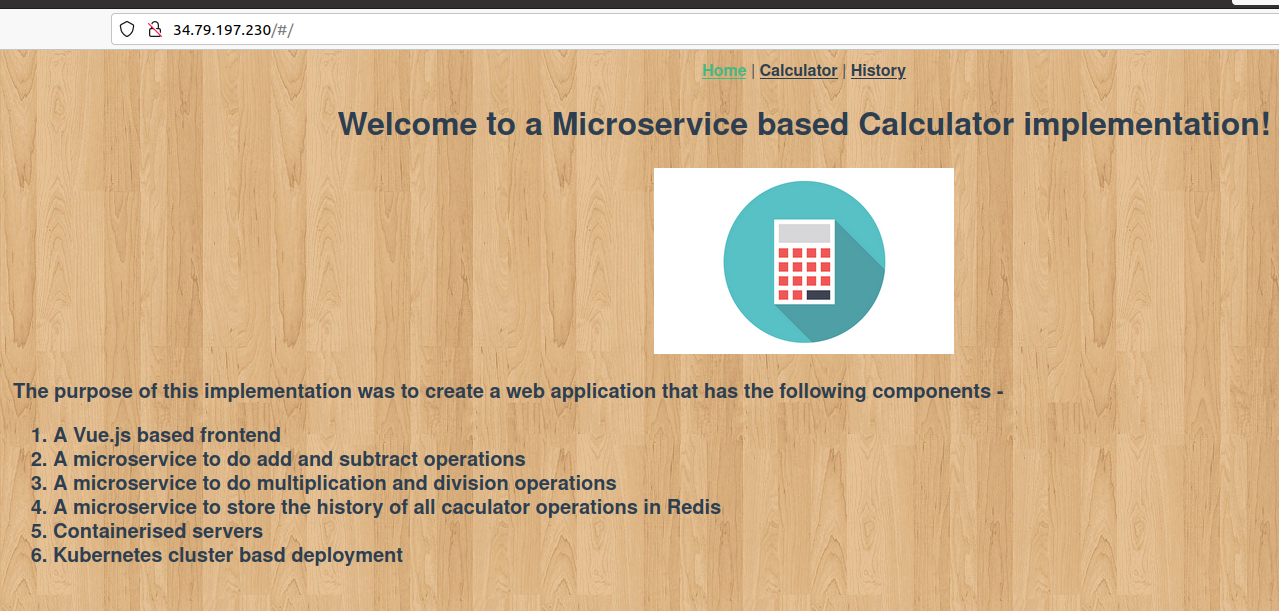
\includegraphics[width=1.0\textwidth]{./pictures/ingresslink.png}
\caption{Application Interface}
\label{fig:Application Interface}
\end{figure}

\begin{itemize}
    \item Access the calculator by clicking on "Calculator" link in to top and the command history by clicking on "History".
\end{itemize}
\begin{figure}[H]
\centering
    \centering
    {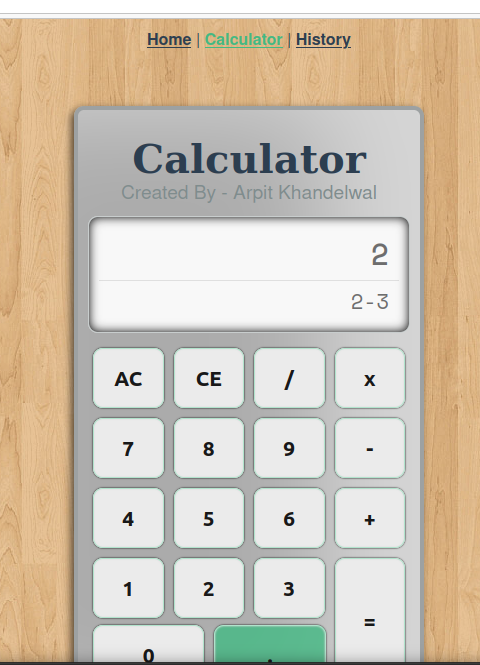
\includegraphics[width=0.4\textwidth]{./pictures/calc.png}}
    {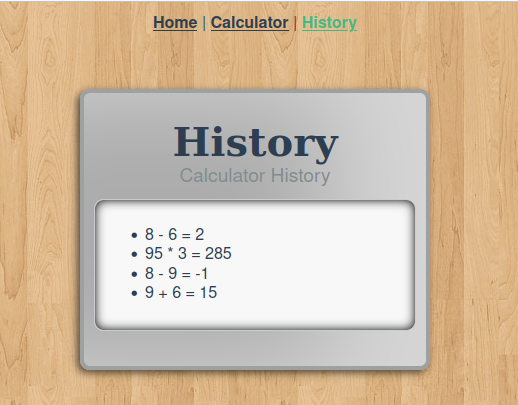
\includegraphics[width=0.4\textwidth]{./pictures/boot.png}}
\caption{Calculator and History}
\label{fig:Service/Bootstorage}
\end{figure}

\clearpage
\section{Monitoring}

\begin{itemize}
    \item Here we can see all the different components of kube-prometheus.
\end{itemize}

\begin{lstlisting} [style=bash]
$ kubectl get all -n kube-prometheus
\end{lstlisting}


\begin{figure}[H]
\centering
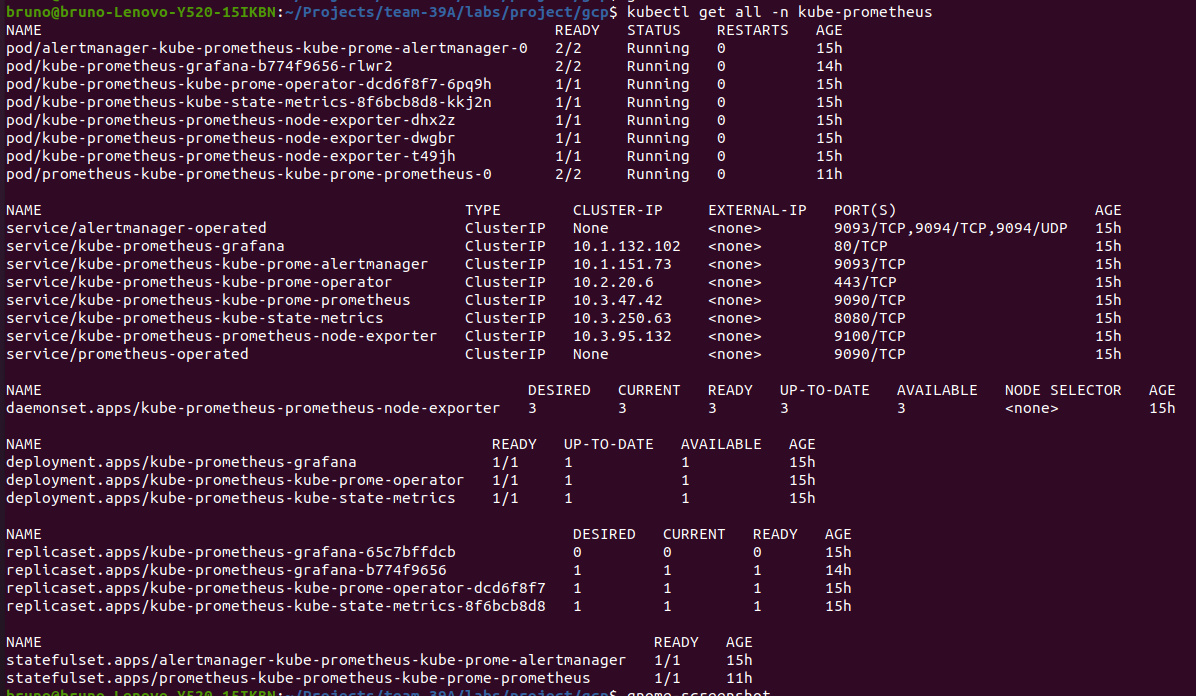
\includegraphics[width=1.0\textwidth]{./pictures/prometheus.png}
\caption{Kube-prometheus}
\label{fig:Kube-prometheus}
\end{figure}

\begin{itemize}
    \item In order to access Grafana, enter the IP address retrieved in last section followed by /grafana. The default username is "admin". In the tool we can access different dashboards to check metrics from our system, which allows for monitoring different aspects of the cluster.
\end{itemize}

\begin{figure}[htb]
\centering
\includegraphics[width=1.0\textwidth]{./pictures/grafkubelets.png}
\caption{Grafana}
\label{fig:Grafana}
\end{figure}

\begin{figure}[htb]
\centering
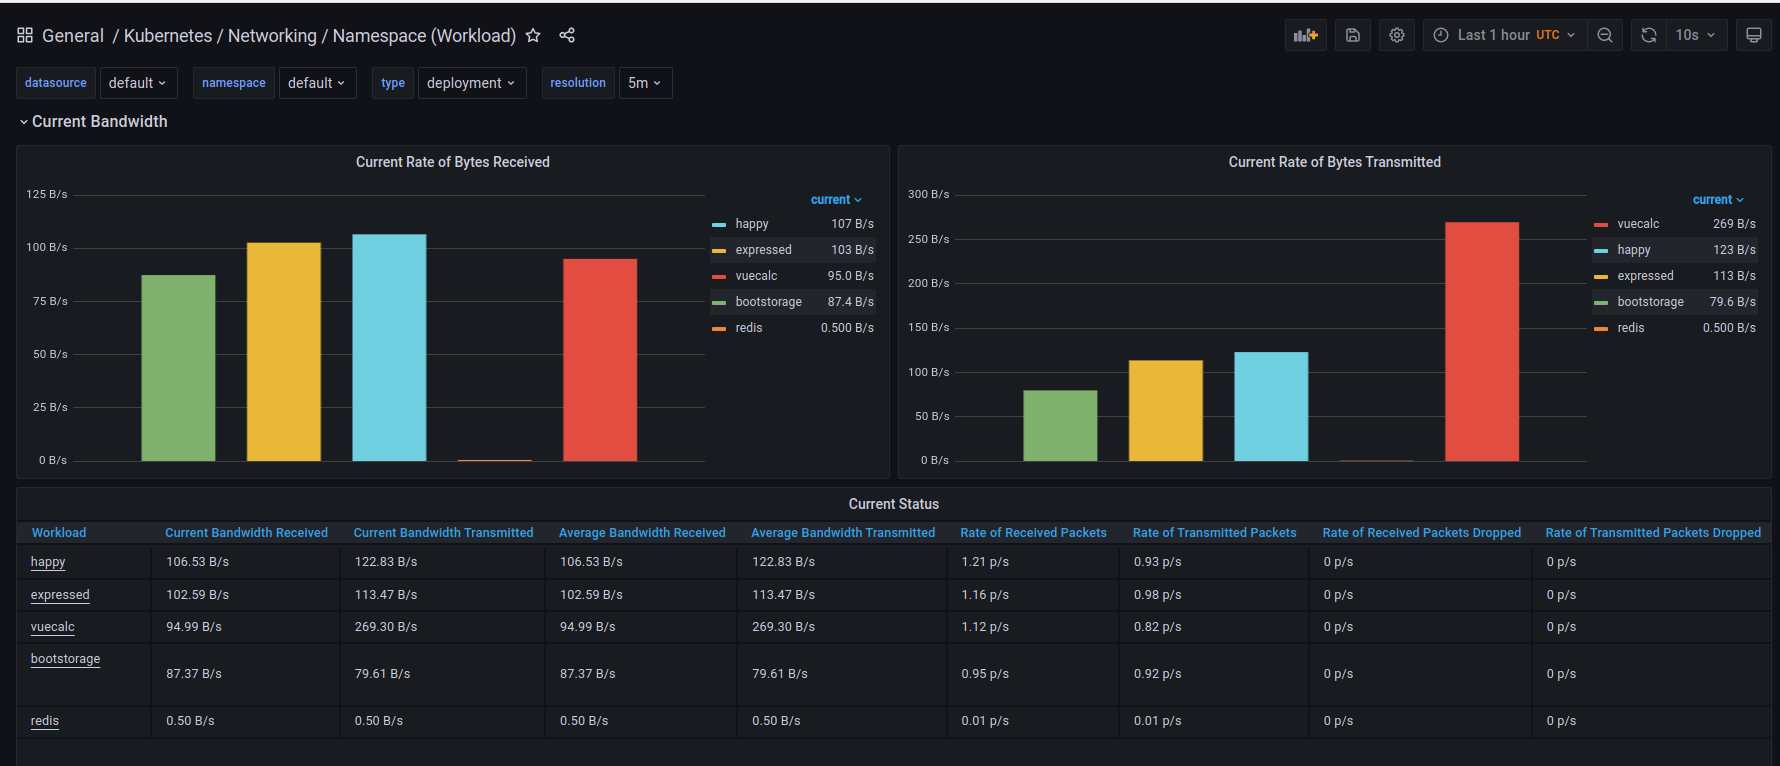
\includegraphics[width=1.0\textwidth]{./pictures/grafanamm.png}
\caption{Grafana Micro-Services Workload}
\label{fig:Grafana Micro-Services Workload}
\end{figure}






\chapter{Final Remarks}

An improvement to be made would be to add TLS to the application, this could be done using \href{https://cert-manager.io/}{Cert-Manager}. 

Another improvement would be to add \href{https://www.nginx.com/products/nginx-service-mesh}{NGINX Service Mesh} to our cluster, this would allow securing the communication between pods, traffic shaping so that when deploying new versions only a small amount of traffic goes to them in case of bugs and better visualization.

Finally our project only has one environment, in a real life case we would have to have multiple, one for development, staging and production.

% #############################################################################
%                        END OF MAIN DOCUMENT BODY
% #############################################################################
% -----------------------------------------------------------------------------
%  Bibliography
% -----------------------------------------------------------------------------
\bibliographystyle{IEEEtran}
% > entries ordered in the order in which the citations appear, with numeric 
% reference markers
% External bibliography database file in the BibTeX format
\cleardoublepage
%\bibliography{IST-UL-Project-Report_bib_DB}
% Add entry in the table of contents as chapter
\addcontentsline{toc}{chapter}{\bibname}
% #############################################################################
\end{document}
% #############################################################################

